\chapter{Indirizzamento IPv4 e Routing}

In questo capitolo affronteremo il funzionamento del protocollo IPv4 (che per semplicità chiameremo spesso solo IP), analizzando nel dettaglio come vengono assegnati gli indirizzi, come sono strutturate le reti e come i router decidono l'inoltro dei pacchetti attraverso il processo di routing.

\section{Il Protocollo IP: Concetti Fondamentali}
Il protocollo IP (Internet Protocol) rappresenta il protocollo di livello di rete dell'architettura TCP/IP (definito nella RFC 791). Il suo compito principale è definire il formato del datagramma, il piano di indirizzamento e le regole di inoltro (forwarding). 

Il protocollo presenta due caratteristiche fondamentali:
\begin{itemize}
    \item \textbf{Connectionless (Senza connessione):} Non viene stabilita alcuna connessione preliminare prima dell'invio dei dati. Ogni datagramma viene inoltrato in modo del tutto indipendente dagli altri. Questo implica che datagrammi appartenenti allo stesso flusso di comunicazione possano seguire percorsi diversi e arrivare a destinazione fuori ordine.
    \item \textbf{Best effort (Miglior sforzo):} La rete fa il possibile per consegnare i datagrammi, ma non offre alcuna garanzia. I datagrammi possono essere persi, duplicati, ritardati o corrotti. Non vi è garanzia sul throughput, sul ritardo, né esistono meccanismi di acknowledgement (conferma di ricezione) o di ritrasmissione a livello IP. Il recupero degli errori, se necessario, è delegato ai protocolli dei sistemi terminali (come il TCP).
\end{itemize}

I router, in questa architettura, mantengono un nucleo semplice: non conservano alcuno stato relativo ai flussi di dati (per-flow state). L'intelligenza della rete è confinata ai margini (negli host). 
Il protocollo IP è inoltre indipendente dalla tecnologia sottostante: può viaggiare su qualsiasi livello di collegamento (Ethernet, Wi-Fi, PPP, ecc.), utilizzando la frammentazione per adattare il datagramma alla MTU (Maximum Transmission Unit) di ciascun link. 
Per la protezione dai loop di instradamento, utilizza il campo TTL (Time To Live), che viene decrementato a ogni salto (hop); se raggiunge lo zero, il pacchetto viene scartato. Dispone infine di protocolli di supporto fondamentali come ICMP (per diagnostica e segnalazione errori) e ARP (per la risoluzione degli indirizzi fisici).

\section{Indirizzamento IPv4}

\subsection{L'Indirizzo IP e le Interfacce di Rete}
Un indirizzo IPv4 è un numero a 32 bit che identifica univocamente a livello globale un'interfaccia di rete. 

È fondamentale precisare, come sottolineato dal professore, che l'indirizzo IP \textbf{non identifica un dispositivo o un utente, ma una specifica interfaccia di rete}. Ad esempio, uno smartphone possiede sia un'interfaccia Wi-Fi sia un'interfaccia per la rete cellulare (es. 5G). Se entrambe sono attive e collegate, lo smartphone disporrà di due indirizzi IP distinti, uno per ciascuna rete. 
Questo concetto è ancora più evidente nei router: un router, per definizione, deve interconnettere almeno due reti diverse, pertanto possiede almeno due interfacce di rete e, di conseguenza, almeno due indirizzi IP.

Per comodità di lettura da parte degli esseri umani, i 32 bit sono divisi in 4 gruppi da 8 bit (4 byte). Ogni byte viene convertito in un numero decimale (da 0 a 255) e separato da un punto. Questa è la classica notazione "dotted-decimal" (es. \texttt{223.1.1.1}).

\subsection{Parte di Rete e Parte di Host}
Per garantire che gli indirizzi siano univoci a livello globale, non è possibile permettere a ciascuno di inventare il proprio indirizzo a 32 bit, altrimenti si creerebbe un'anarchia ingestibile. La soluzione adottata è strutturare l'indirizzo IP in modo gerarchico, dividendolo in due parti logiche:
\begin{itemize}
    \item \textbf{Network part (Parte di Rete):} I bit più significativi (a sinistra). Identifica la rete fisica o logica a cui il dispositivo è connesso.
    \item \textbf{Host part (Parte di Host):} I bit meno significativi (a destra). Identifica la specifica interfaccia all'interno di quella rete.
\end{itemize}

Tutti i dispositivi (o meglio, le interfacce) connessi alla medesima rete fisica condividono la stessa \emph{network part}. Questo approccio semplifica l'assegnazione: un ente centrale assegna un prefisso di rete a un'organizzazione (es. il Politecnico), e tale organizzazione sarà libera di amministrare localmente la \emph{host part} per i propri dispositivi, garantendo scalabilità e unicità globale senza la necessità di un controllo centrale su ogni singolo dispositivo.

\subsection{Indirizzi Speciali}
All'interno dello spazio di indirizzamento, alcune combinazioni sono riservate a scopi specifici e non possono essere assegnate alle interfacce degli host:

\begin{itemize}
    \item \textbf{Network ID (Identificativo di rete):} Ha una determinata parte di rete e \textbf{tutti 0} nella parte di host. Rappresenta la rete stessa e non può essere assegnato a nessun dispositivo.
    
    \begin{figure}[H]
        \centering
        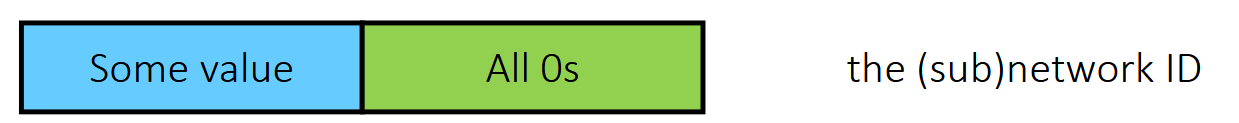
\includegraphics[width=0.5\textwidth]{capitoli/01a - IPv4-Summary/images/network_id.png}
    \end{figure}

    \item \textbf{Directed Broadcast (Broadcast di rete):} Ha una determinata parte di rete e \textbf{tutti 1} nella parte di host. Rappresenta tutti gli host appartenenti a quella specifica sottorete. Concettualmente, un pacchetto inviato a questo indirizzo dovrebbe raggiungere tutti i nodi di quella rete. Tuttavia, per evitare abusi o attacchi informatici, i router degli operatori (ISP) di solito bloccano i pacchetti di directed broadcast provenienti da reti esterne.
    \begin{figure}[H]
        \centering
        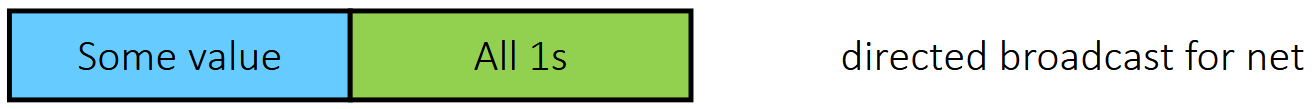
\includegraphics[width=0.5\textwidth]{capitoli/01a - IPv4-Summary/images/directed_broadcast.png}
    \end{figure}
    \item \textbf{Limited Broadcast:} Un indirizzo composto interamente da 1 (\texttt{255.255.255.255}). Serve per inviare un messaggio in broadcast esclusivamente nella rete locale fisica in cui ci si trova. Il router non innesterà mai questo pacchetto in altre reti.
    \begin{figure}[H]
        \centering
        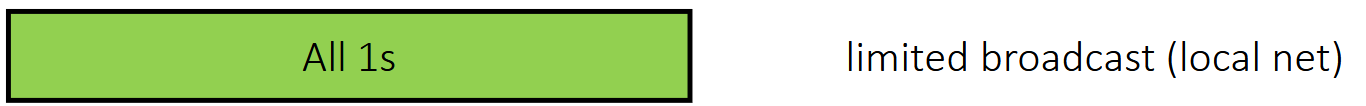
\includegraphics[width=0.5\textwidth]{capitoli/01a - IPv4-Summary/images/limited_broadcast.png}
    \end{figure}
    \item \textbf{Loopback (\texttt{127.x.x.x}):} Indirizzi il cui primo byte è 127 (il più famoso è \texttt{127.0.0.1}). Identificano la macchina locale (localhost). Questo indirizzo è estremamente utile per i programmatori: permette a processi software in esecuzione sulla stessa macchina (es. un server web e un database) di comunicare tra loro utilizzando lo stack IP senza che il traffico esca effettivamente sulla rete fisica.
    \begin{figure}[H]
        \centering
        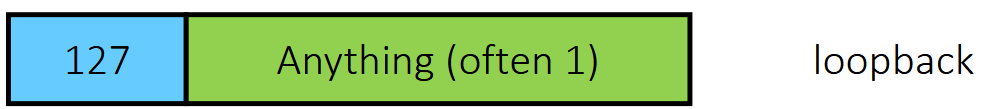
\includegraphics[width=0.45\textwidth]{capitoli/01a - IPv4-Summary/images/loopback.png}
    \end{figure}
\end{itemize}

\subsection{Classful Addressing (Approccio Storico)}
Inizialmente, per far capire ai router dove finisse la parte di rete e iniziasse la parte di host, Internet utilizzava il concetto di "Classi" (Classful Addressing). Il confine era rigidamente fissato in base ai primi bit dell'indirizzo:

\begin{itemize}
    \item \textbf{Classe A:} Il primo bit è \texttt{0}. La parte di rete occupa 8 bit (1 byte), la parte di host 24 bit. Permetteva $2^{24}$ interfacce. Indirizzi pensati per organizzazioni gigantesche (es. grandi operatori).
    \begin{figure}[H]
        \centering
        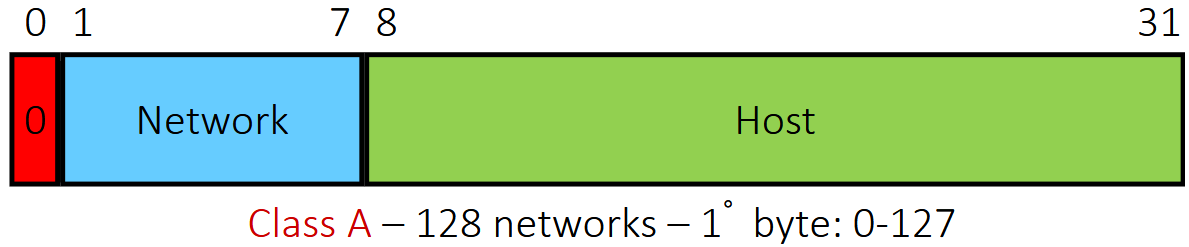
\includegraphics[width=0.5\textwidth]{capitoli/01a - IPv4-Summary/images/class_a.png}
    \end{figure}
    \item \textbf{Classe B:} I primi bit sono \texttt{10}. La parte di rete occupa 16 bit, la parte di host 16 bit. Permetteva $2^{16}$ (circa 65.000) interfacce.
    \begin{figure}[H]
        \centering
        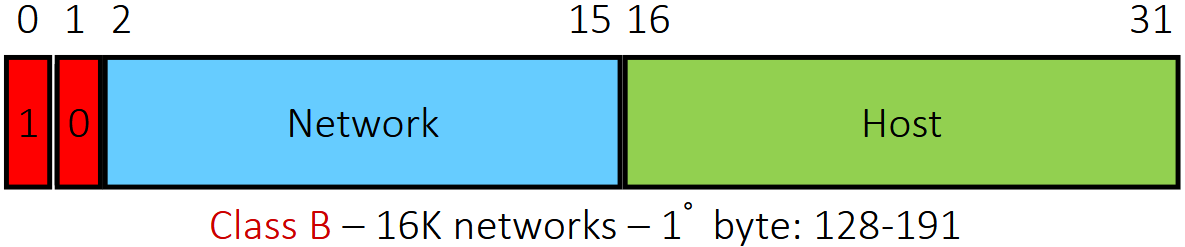
\includegraphics[width=0.5\textwidth]{capitoli/01a - IPv4-Summary/images/class_b.png}
    \end{figure}
    \item \textbf{Classe C:} I primi bit sono \texttt{110}. La parte di rete occupa 24 bit, la parte di host 8 bit. Permetteva $2^8 = 256$ interfacce (in realtà 254 assegnabili). Pensata per reti medio-piccole.
    \begin{figure}[H]
        \centering
        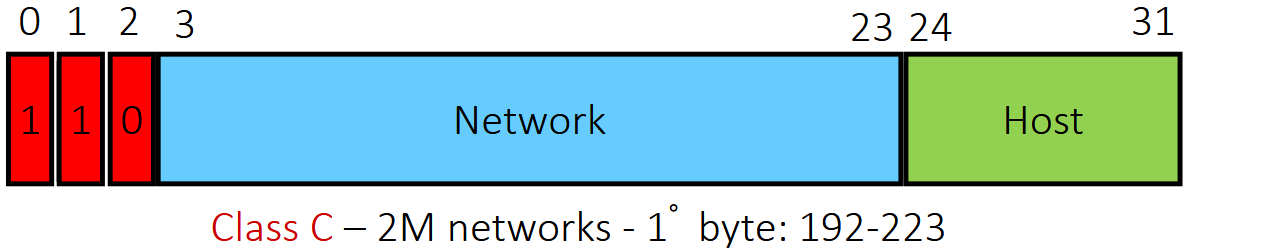
\includegraphics[width=0.5\textwidth]{capitoli/01a - IPv4-Summary/images/class_c.png}
    \end{figure}
\end{itemize}



Il vantaggio di questo metodo era la velocità hardware: un router doveva controllare solo i primissimi bit per capire la struttura dell'indirizzo. 
\textbf{Il problema:} Non era scalabile ed era estremamente rigido. Come sottolineato dal professore, se un'organizzazione aveva bisogno di 300 indirizzi, la Classe C (254 host) era insufficiente. L'organizzazione era costretta ad acquistare una Classe B, bloccando di fatto $65.000$ indirizzi, la maggior parte dei quali non sarebbe mai stata utilizzata (il Politecnico, ad esempio, acquistò un'intera rete \texttt{130.192.0.0/16} sprecando moltissimi indirizzi).

\subsection{CIDR: Classless InterDomain Routing e Netmask}
Per ovviare agli sprechi delle classi, è stato introdotto il \textbf{CIDR}, che elimina il concetto di classe. La lunghezza della porzione di rete diventa variabile.
Per indicare dove avviene la separazione, si utilizzano due notazioni equivalenti:

\begin{enumerate}
    \item \textbf{Prefix Length (Lunghezza del prefisso):} Si aggiunge all'indirizzo una barra e il numero di bit che compongono la parte di rete (\texttt{/x}). Ad esempio, \texttt{200.23.16.0/23} indica che i primi 23 bit identificano la rete, e i restanti $32-23=9$ bit identificano l'host.
    \item \textbf{Netmask (Maschera di sottorete):} Un numero a 32 bit composto da tanti "1" quanti sono i bit della parte di rete, seguiti da tutti "0" per la parte di host. L'indirizzo \texttt{/23} di prima, in binario ha i primi 23 bit a 1, e i restanti 9 a 0, che convertito in notazione decimale puntata diventa \texttt{255.255.254.0}.
\end{enumerate}

\begin{figure}[H]
    \centering
    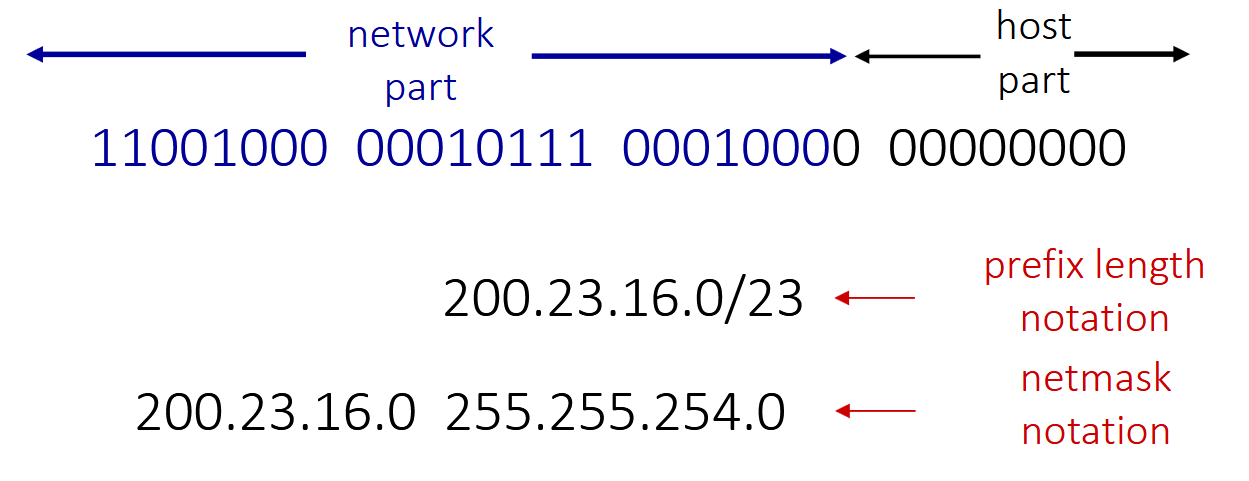
\includegraphics[width=0.7\textwidth]{capitoli/01a - IPv4-Summary/images/netmask.png}
    \caption{Indirizzo IPv4 in binario, suddiviso in parte di rete e parte di host, con la corrispondente notazione Prefix Length (\texttt{/23}) e Netmask (\texttt{255.255.254.0}).}
    \label{fig:netmask}
\end{figure}

\textbf{Perché si usa la Netmask?} Come evidenziato a lezione, sebbene per noi umani la notazione \texttt{/x} sia più chiara, i sistemi operativi e l'hardware dei router preferiscono la netmask. Questo perché la netmask permette di ricavare l'identificativo di rete di un indirizzo IP eseguendo una semplice e rapidissima operazione logica di \textbf{AND bit-a-bit} tra l'indirizzo IP e la netmask stessa.

Di seguito una comoda tabella per la conversione rapida del byte "spezzato" della netmask:

\begin{table}[H]
    \centering
    \begin{tabular}{c c c}
        \toprule
        \textbf{Bit a '1' nel byte} & \textbf{Valore Binario} & \textbf{Valore Decimale} \\
        \midrule
        0 & 0000 0000 & 0 \\
        1 & 1000 0000 & 128 \\
        2 & 1100 0000 & 192 \\
        3 & 1110 0000 & 224 \\
        4 & 1111 0000 & 240 \\
        5 & 1111 1000 & 248 \\
        6 & 1111 1100 & 252 \\
        7 & 1111 1110 & 254 (non valido nell'ultimo byte per reti normali)\\
        8 & 1111 1111 & 255 (identifica il singolo host, \texttt{/32}) \\
        \bottomrule
    \end{tabular}
    \caption{Possibili valori di una Netmask per un singolo byte.}
    \label{tab:netmask}
\end{table}

\subsection{Dimensionamento delle Sottoreti (Subnetting)}
Ogni sottorete (subnet) deve essere definita da un \textit{Network ID} valido. Un Network ID è valido solo se \textbf{tutti i bit della parte di host sono a zero}. 
Ad esempio, se analizziamo \texttt{130.192.1.4/29}, i bit di host sono 3 ($32-29$). Il numero 4 in binario sui 3 bit finali si scrive \texttt{100}, che non è tutto zero. Quindi \texttt{130.192.1.4/29} è un IP assegnabile a un host, ma non è un identificativo di rete valido.

In una generica rete con una parte di host di $n$ bit, il numero di indirizzi IP totali è $2^n$. Tuttavia, il numero di \textbf{indirizzi effettivamente assegnabili alle interfacce} è:
\[ Indirizzi\_assegnabili = 2^n - 2 \]
Questo perché si devono scartare il primo indirizzo (tutti zero = Network ID) e l'ultimo indirizzo (tutti uno = Broadcast).

\begin{remark}[Reti Point-to-Point e il caso del /31]
Nelle connessioni dirette tra due router (Point-to-Point), sono necessari solo 2 indirizzi IP (uno per lato). Una rete \texttt{/30} fornisce 2 bit di host, quindi $2^2 = 4$ IP totali, da cui se ne sottraggono 2, lasciando esattamente 2 IP assegnabili.
Esiste un'RFC che permette di utilizzare reti \texttt{/31} (solo 2 IP totali) per i link point-to-point, sacrificando volutamente il Network ID e l'indirizzo di Broadcast. Tuttavia, come precisato dal docente, per evitare complicazioni o malfunzionamenti in determinati scenari, \textbf{in questo corso si assumerà che la sottorete più piccola utilizzabile per un link point-to-point sia la \texttt{/30}}. Qualsiasi prefisso maggiore di 30 (es. \texttt{/31} o \texttt{/32}) non è considerato una sottorete valida.
\end{remark}

\section{Il Routing IP}

Quando un router riceve un datagramma IP, deve decidere su quale porta inoltrarlo. Questa decisione viene presa analizzando la \textbf{Tabella di Routing} e utilizzando un principio fondamentale.

\subsection{Longest Prefix Matching (LPM)}
Il router esegue un confronto riga per riga tra l'Indirizzo IP di Destinazione contenuto nel pacchetto e la Network ID di ciascuna riga, calcolando il match tramite operazione di \textbf{AND logico} con la Netmask.

Se la destinazione fa match con più di una riga, il router seleziona la riga il cui match è avvenuto sul numero maggiore di bit della parte di rete. Questo meccanismo prende il nome di \textbf{Longest Prefix Matching} (corrispondenza del prefisso più lungo). Il principio è intuitivo: un prefisso più lungo indica una destinazione più specifica.

\begin{example}[Esempio di Longest Prefix Matching]
Supponiamo che il router riceva un pacchetto destinato all'indirizzo IP \texttt{200.23.17.1}. 
La tabella di routing presenta due voci:
\begin{enumerate}
    \item \texttt{200.23.16.0/20}
    \item \texttt{200.23.16.0/23}
\end{enumerate}
Il router opera in binario lavorando in particolare sul terzo byte (l'unico che subisce il partizionamento, dato che il prefisso è compreso tra 16 e 24).
L'indirizzo di destinazione sul terzo byte ha valore $17$, che in binario è \texttt{00010001}.

\textbf{Test contro la riga 1 (/20):}
La netmask di un \texttt{/20} sul terzo byte lascia 4 bit di rete e 4 bit di host, e vale $240$ (\texttt{11110000}).
Facendo l'AND logico bit a bit tra il byte di destinazione e la maschera otteniamo:
\begin{center}
\texttt{00010001} (17) AND \\
\texttt{11110000} (240) = \\
\texttt{00010000} (16)
\end{center}
Il risultato ($16$) coincide col valore di rete indicato nella riga della tabella. Abbiamo un match su 20 bit.

\textbf{Test contro la riga 2 (/23):}
La netmask di un \texttt{/23} lascia 7 bit di rete e 1 bit di host, e vale $254$ (\texttt{11111110}).
\begin{center}
\texttt{00010001} (17) AND \\
\texttt{11111110} (254) = \\
\texttt{00010000} (16)
\end{center}
Anche in questo caso otteniamo 16. Abbiamo un match su 23 bit.

Poiché ci sono due match, il router applicherà la regola del Longest Prefix Matching, scegliendo la \textbf{riga 2} perché il prefisso (\texttt{/23}) è più lungo e quindi più specifico rispetto a \texttt{/20}.
\end{example}

Questo meccanismo di ricerca lineare (valutare tutte le entry per trovare il prefisso più lungo) evidenzia perché nei router le tabelle di routing devono essere ottimizzate: l'hardware deve compiere queste operazioni a velocità altissime per ogni singolo pacchetto in transito.

\subsection{Struttura della Tabella di Routing}
Una tabella di routing completa fornisce, per ogni destinazione, non solo il link di uscita, ma anche l'indirizzo del \textbf{Next Hop} (salto successivo), ovvero l'indirizzo IP dell'interfaccia del prossimo router a cui consegnare il pacchetto.

Le rotte in tabella si dividono principalmente in due categorie (indicate spesso con una sigla o un tipo):
\begin{itemize}
    \item \textbf{C (Connected) - Direttamente Connesse:} Sono le reti fisicamente collegate alle interfacce del router. In questo caso il router non ha bisogno di un "next hop" intermedio (altri router) per raggiungerle; il pacchetto viene inviato direttamente sul link di uscita (e il MAC address finale viene risolto tramite protocollo ARP). L'interfaccia locale viene spesso indicata nel campo Next Hop.
    \item \textbf{S (Static) - Rotte Statiche:} Configurate manualmente dall'operatore di rete.
\end{itemize}

\textbf{La metrica o Costo (Cost / Weight):}
Come decide l'operatore quali percorsi inserire? Se una subnet è raggiungibile tramite due percorsi diversi (ad esempio un percorso che attraversa un solo router ma usa cavi lenti, e un percorso che attraversa due router ma in fibra ottica veloce), a ogni link viene associato un \textit{peso} o costo. Tramite algoritmi di ottimizzazione (es. Dijkstra), si individua lo \textit{Shortest Path} (il percorso a costo minimo). La tabella di routing conterrà la rotta con il costo complessivo inferiore.
Il costo è inoltre utilissimo per gestire guasti: è possibile inserire nella tabella due rotte verso la stessa destinazione, assegnando a una delle due un costo artificiosamente più alto (es. 5 contro 1). Finché la rotta a costo 1 è attiva, il router userà quella; se il link principale subisce un guasto, la rotta principale verrà eliminata e il router comincerà a utilizzare il percorso di backup a costo 5, garantendo continuità di servizio.

\textbf{La Default Route (Rotta di Default):}
Spesso indicata come \texttt{0.0.0.0/0}. È una rotta fondamentale per l'accesso a Internet. 
Dal punto di vista matematico, un \texttt{/0} richiede un match su 0 bit. Questo significa che l'operazione di AND è inutile: \textbf{qualsiasi} indirizzo IP di destinazione farà match con questa riga. Tuttavia, a causa del Longest Prefix Matching, questa rotta verrà utilizzata dal router \textbf{esclusivamente} se nessun'altra rotta più specifica presente in tabella ha fatto match. In genere, il Next Hop della default route è l'indirizzo IP del router dell'ISP (Internet Service Provider) a cui la rete aziendale è collegata, fungendo da "scivolo" verso l'esterno per tutto il traffico sconosciuto.

\subsection{Esempio Pratico e Ottimizzazione (Route Aggregation)}

% FIGURA ORIGINALE DA RECUPERARE DALLE SLIDE
% Slide di provenienza: 15
% Tipo: schema
% Descrizione: Topologia di rete con router R1, R2, R3, reti locali associate, link punto-punto e connessione verso Internet.
% Punto di inserimento: Qui, per comprendere l'esempio della routing table sottostante.
% File da inserire: placeholder_topologia_routing

\begin{figure}[H]
    \centering
    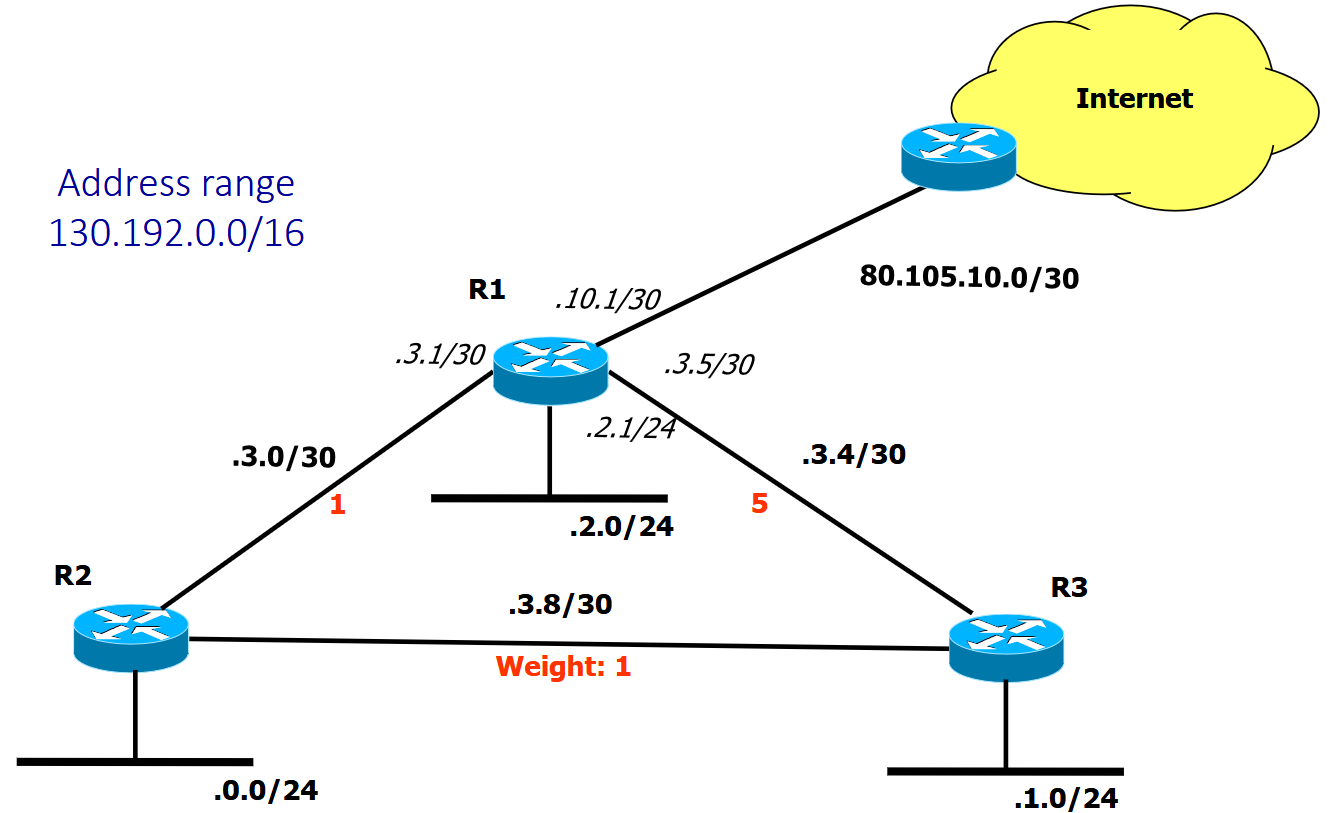
\includegraphics[width=0.7\textwidth]{capitoli/01a - IPv4-Summary/images/placeholder_topologia_routing}
    \caption{Topologia della rete per la costruzione della tabella di routing di R1.}
    \label{fig:topologia}
\end{figure}

Prendiamo in esame un caso pratico in cui il router \textbf{R1} appartiene a un'organizzazione (es. Politecnico) a cui è stato assegnato il range \texttt{130.192.0.0/16}. R1 è collegato a varie subnet interne, a router vicini (R2, R3) e a Internet tramite un Default Gateway.

Una prima versione corretta della Tabella di Routing di R1 per le reti non direttamente connesse potrebbe essere la seguente:

\begin{table}[H]
    \centering
    \begin{tabular}{c l l c}
        \toprule
        \textbf{Tipo} & \textbf{Destinazione} & \textbf{Next-hop} & \textbf{Costo} \\
        \midrule
        S & 130.192.0.0/24 & 130.192.3.2 (R2) & 1 \\
        S & 130.192.1.0/24 & 130.192.3.2 (R2) & 2 \\
        S & 130.192.3.8/30 & 130.192.3.2 (R2) & 1 \\
        S & 0.0.0.0/0      & 80.105.10.2 (ISP) & 1 \\
        \bottomrule
    \end{tabular}
    \caption{Porzione della tabella di routing di R1 (rotte statiche).}
    \label{tab:routing_r1}
\end{table}

\textbf{Ottimizzazione mediante Route Aggregation:}
Come sottolineato dal docente, la tabella vista sopra funziona perfettamente ma non è ottimizzata. L'LPM scala in modo lineare (Lento). Per accelerare i calcoli, i router raggruppano le rotte contigue con lo stesso Next Hop, un processo noto come \textit{Route Aggregation} (o supernetting).

Notiamo che le prime due righe indirizzano il traffico verso lo stesso Next Hop (R2). Invece di usare due \texttt{/24}, possiamo aggregarle riducendo i bit di rete.
Abbiamo diverse scelte, ognuna con dei trade-off illustrati a lezione:
\begin{enumerate}
    \item \textbf{Aggregazione totale (\texttt{130.192.0.0/16}):} Indirizza verso R2 tutto il traffico interno dell'organizzazione. Questo garantisce il minimo numero di righe nella tabella, ma è un approccio \textit{pericoloso}: se domani viene aggiunta una nuova rete aziendale da un'altra parte (es. connessa a R3), l'indirizzo verrà intercettato da questo \texttt{/16} e il traffico andrà perso verso R2 anziché verso R3. 
    \item \textbf{Aggregazione parziale \texttt{/22} (\texttt{130.192.0.0/22}):} Copre gli indirizzi dal \texttt{0.0} al \texttt{3.255}. Riduce i rischi rispetto al \texttt{/16}, includendo solo pochi indirizzi al momento non allocati.
    \item \textbf{Aggregazione stretta \texttt{/23} (\texttt{130.192.0.0/23}):} È l'approccio più sicuro in questo contesto. Copre esattamente e unicamente \texttt{130.192.0.0/24} e \texttt{130.192.1.0/24}. Mantiene la tabella snella senza includere alcun indirizzo non esplicitamente presente nella topologia attuale.
\end{enumerate}

Sostituendo le prime due righe con la singola riga \texttt{130.192.0.0/23} avente Next Hop \texttt{130.192.3.2}, il router impiegherà meno tempo computazionale, mantenendo invariata la correttezza dell'inoltro.